\documentclass[11pt,aspectratio=169]{beamer}

% ---------------------------------------------------------------
% Pure black & white theme
% ---------------------------------------------------------------
\usetheme{default}
\usecolortheme{seagull}
\setbeamercolor{background canvas}{bg=white}
\setbeamercolor{normal text}{fg=black, bg=white}
\setbeamercolor{frametitle}{fg=black, bg=white}
\setbeamercolor{title}{fg=black}
\setbeamercolor{subtitle}{fg=black!70}
\setbeamercolor{author}{fg=black!70}
\setbeamercolor{date}{fg=black!70}
\setbeamercolor{item}{fg=black}
\setbeamertemplate{itemize item}{\textbullet}
\setbeamertemplate{itemize subitem}{--}
\setbeamertemplate{navigation symbols}{}
\setbeamerfont{frametitle}{series=\bfseries, size=\large}

\usepackage{tikz}
\usetikzlibrary{shapes, arrows.meta, positioning, calc, fit,
                backgrounds, decorations.pathmorphing}
\usepackage{microtype}

% ---------------------------------------------------------------
\tikzset{
  pi/.style={
    rectangle, draw=black, fill=white, thick, rounded corners=2pt,
    minimum width=1.9cm, minimum height=0.85cm,
    align=center, font=\footnotesize\ttfamily, inner sep=2pt,
  },
  pibig/.style={
    rectangle, draw=black, fill=white, thick, rounded corners=2pt,
    minimum width=2.6cm, minimum height=1.1cm,
    align=center, font=\footnotesize\ttfamily, inner sep=3pt,
  },
  anchor pi/.style={pibig, fill=black!12},
  sensor/.style={
    rectangle, draw=black, fill=white, thick,
    minimum width=1.6cm, minimum height=0.55cm,
    align=center, font=\scriptsize, inner sep=2pt,
  },
  cell/.style={
    ellipse, draw=black, very thick, dashed, fill=black!3,
    align=center, font=\footnotesize\ttfamily,
  },
  meshlink/.style={
    line width=0.9pt, draw=black,
    decorate, decoration={snake, amplitude=0.5mm, segment length=3mm},
  },
  meshlink weak/.style={
    line width=0.5pt, draw=black!45, dashed,
  },
  arrow/.style={
    -{Latex[length=2.5mm]}, line width=0.8pt, draw=black,
  },
  fatarrow/.style={
    -{Latex[length=3.5mm]}, line width=1.6pt, draw=black,
  },
  tlabel/.style={
    font=\scriptsize\itshape, align=center,
  }
}

% ---------------------------------------------------------------
\title{EweGo Mesh Networking}
\subtitle{Self-organizing field network for multimodal sensor arrays}
\date{May 2026}

\begin{document}

% ===============================================================
\begin{frame}[plain]
  \titlepage
\end{frame}

% ===============================================================
\begin{frame}{A self-organizing mesh in the field}

\begin{columns}[T,onlytextwidth]

\column{0.42\textwidth}
\vspace{0.3cm}

No router. No AP. No internet.

\medskip
Each Pi powers on and joins automatically. The mesh self-heals when sheep wander out of range.

\medskip
\textbf{B.A.T.M.A.N.-adv over IBSS}\\
L2 kernel routing on top of 802.11 ad-hoc. The whole mesh shows up as one virtual interface, \texttt{bat0}.

\column{0.55\textwidth}
\centering
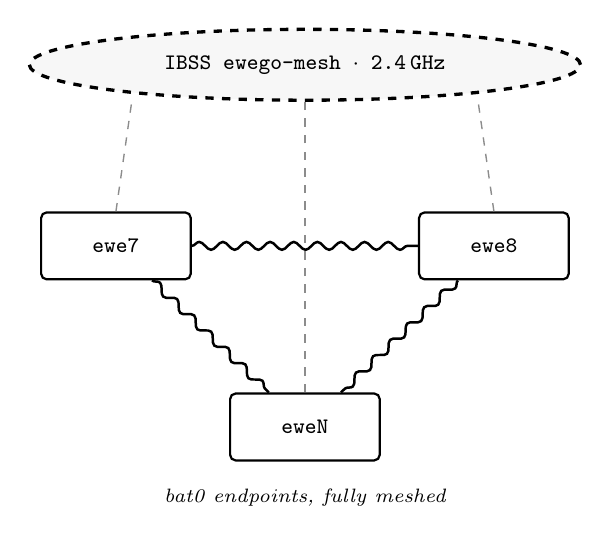
\begin{tikzpicture}[scale=1.0]

  \node[cell, minimum width=7cm, minimum height=0.9cm] (cell) at (0, 3.0)
    {IBSS \texttt{ewego-mesh} $\cdot$ 2.4\,GHz};

  \node[pi] (a) at (-2.4, 0.7) {ewe7};
  \node[pi] (b) at ( 2.4, 0.7) {ewe8};
  \node[pi] (c) at ( 0.0,-1.6) {eweN};

  \draw[meshlink] (a) -- (b);
  \draw[meshlink] (a) -- (c);
  \draw[meshlink] (b) -- (c);

  \draw[meshlink weak] (a.north) -- ($(cell.south)+(-2.2,0)$);
  \draw[meshlink weak] (b.north) -- ($(cell.south)+(+2.2,0)$);
  \draw[meshlink weak] (c.north) -- (cell.south);

  \node[tlabel] at (0, -2.5) {bat0 endpoints, fully meshed};

\end{tikzpicture}

\end{columns}
\end{frame}

% ===============================================================
\begin{frame}{Why this is interesting}

\centering
\vspace{0.6cm}

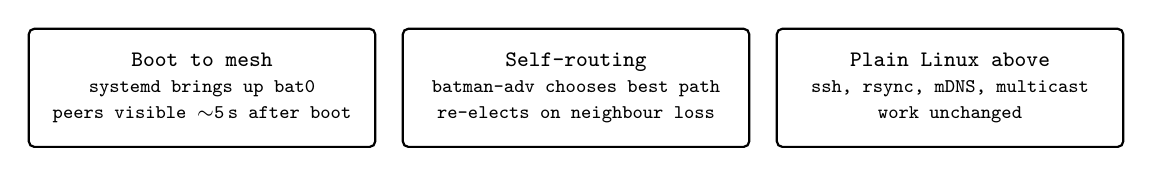
\begin{tikzpicture}[scale=0.95]

  \node[pibig, minimum width=4.4cm, minimum height=1.5cm] (a) at (-5, 0)
    {\textbf{Boot to mesh}\\\scriptsize systemd brings up bat0\\\scriptsize peers visible $\sim$5\,s after boot};

  \node[pibig, minimum width=4.4cm, minimum height=1.5cm] (b) at ( 0, 0)
    {\textbf{Self-routing}\\\scriptsize batman-adv chooses best path\\\scriptsize re-elects on neighbour loss};

  \node[pibig, minimum width=4.4cm, minimum height=1.5cm] (c) at ( 5, 0)
    {\textbf{Plain Linux above}\\\scriptsize ssh, rsync, mDNS, multicast\\\scriptsize work unchanged};

\end{tikzpicture}

\vspace{0.8cm}

\begin{center}
\begin{minipage}{0.85\textwidth}\centering
\large
A handful of Pis in a paddock become a coherent
network --- no commissioning, no central node, no failure choke point.
\end{minipage}
\end{center}
\end{frame}

% ===============================================================
\begin{frame}{Time sync and control across the herd}

\begin{columns}[T,onlytextwidth]

\column{0.45\textwidth}
\vspace{0.2cm}

\textbf{Clocks aligned to $\sim$100--200\,\textmu s}\\
chrony peers over the mesh. Anchor from GPS\,/\,PPS or any one Pi's local clock.

\medskip
\textbf{Synchronized triggers}\\
A common time $\Rightarrow$ ``everyone start recording at T+5\,s'' just works.

\medskip
\textbf{Native broadcast and discovery}\\
mDNS over \texttt{bat0}, batman-adv neighbour table, multicast. Failures detected within $\sim$5\,s.

\column{0.50\textwidth}
\centering
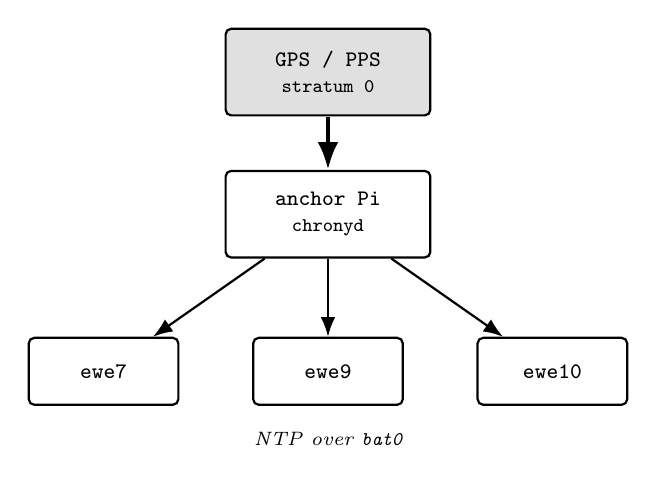
\begin{tikzpicture}[scale=0.95]

  \node[anchor pi]  (gps)  at (0, 2.6)  {GPS / PPS\\\scriptsize stratum 0};
  \node[pibig]      (anc)  at (0, 0.7)  {anchor Pi\\\scriptsize chronyd};
  \node[pi]         (p7)   at (-3.0,-1.4){ewe7};
  \node[pi]         (p9)   at ( 0.0,-1.4){ewe9};
  \node[pi]         (p10)  at ( 3.0,-1.4){ewe10};

  \draw[fatarrow] (gps) -- (anc);
  \draw[arrow]    (anc) -- (p7);
  \draw[arrow]    (anc) -- (p9);
  \draw[arrow]    (anc) -- (p10);

  \node[tlabel] at (0,-2.3) {NTP over \texttt{bat0}};

\end{tikzpicture}

\end{columns}
\end{frame}

% ===============================================================
\begin{frame}{The outcome --- autosynching multimodal sensor arrays}

\centering
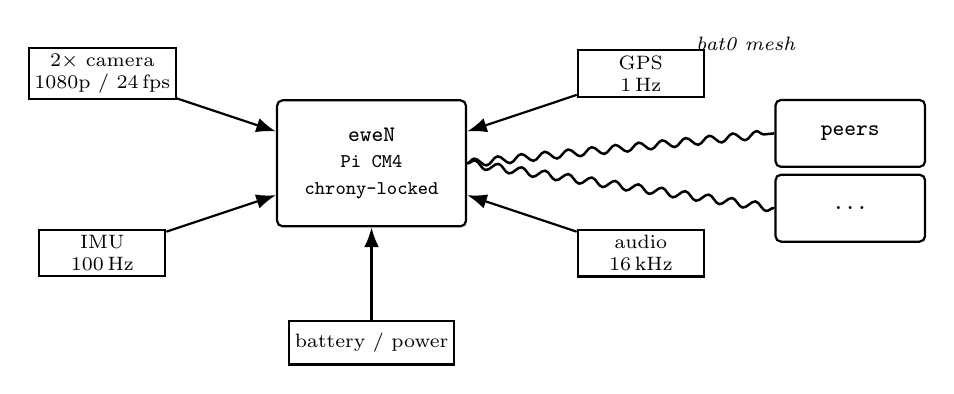
\begin{tikzpicture}[scale=0.95]

  % One Pi as the canonical "sensor node"
  \node[pibig, minimum width=2.4cm, minimum height=1.6cm] (pi) at (0, 0)
    {\textbf{eweN}\\\scriptsize Pi CM4\\\scriptsize chrony-locked};

  % Sensors around the Pi
  \node[sensor] (cam) at (-3.6, 1.2) {2$\times$ camera\\\scriptsize 1080p / 24\,fps};
  \node[sensor] (imu) at (-3.6,-1.2) {IMU\\\scriptsize 100\,Hz};
  \node[sensor] (gps) at ( 3.6, 1.2) {GPS\\\scriptsize 1\,Hz};
  \node[sensor] (aud) at ( 3.6,-1.2) {audio\\\scriptsize 16\,kHz};
  \node[sensor] (bat) at ( 0.0,-2.4) {battery / power};

  \draw[arrow] (cam) -- (pi);
  \draw[arrow] (imu) -- (pi);
  \draw[arrow] (gps) -- (pi);
  \draw[arrow] (aud) -- (pi);
  \draw[arrow] (bat) -- (pi);

  % Mesh peers off to the right
  \node[pi] (p2) at (6.4, 0.4) {peers};
  \node[pi] (p3) at (6.4,-0.6) {\dots};

  \draw[meshlink] (pi.east) -- (p2.west);
  \draw[meshlink] (pi.east) -- (p3.west);
  \node[tlabel] at (5.0, 1.6) {bat0 mesh};

\end{tikzpicture}

\vspace{0.4cm}
\centering
\begin{minipage}{0.9\textwidth}\centering
Every sample on every Pi is timestamped against a common clock to within
$\sim$100\,\textmu s --- across cameras, IMU, audio, GPS, and across animals ---
so cross-modal and cross-sheep correlation is a query on aligned data, not a
calibration problem.
\end{minipage}

\end{frame}

\end{document}
